\section{QUADaps Software}
Um die besondere Detektor-, und diverse Probengeometrien zu simulieren wurde die Simulationssoftware \textbf{QUADaps} nach den 4 Detektorzellen (\textbf{QUAD}) sowie \glqq\textbf{a}bsorption \textbf{p}ath \textbf{s}imulations\grqq entwickelt. Dabei basieren die Berechnungen und Simulationen auf dem Softwarepaket \textit{xrfLibrary}, welches von der AG Kanngießer (TU Berlin) entwickelt wurde. Als Datenbanksatz wird die Elam Datenbank aus dem Paket \textit{xrlfupa} genutzt. Dieses enthält die fundamentalen Röntgenstrahlungsparameter und einen großen Datensatz an optischen Parametern. Mithilfe der \textit{xrfLibrary} werden dann Quellen (\textit{source()}), Proben (\textit{specimen()}), Filter (\textit{filter()}) und Detektoren (\textit{detector()}) definiert. Um eine Fluoreszenzsimulation zu erstellen wird zunächst eine monochromatische Quelle (\textit{monoSource()}) erstellt und ihr die gewünschte Photonenenergie $E$ und Intensität $I_{0}$ übergeben. \newline
Daraufhin muss die zu untersuchende Struktur erstellt werden. Dazu dient ein xy-Raster (\textit{layoutXY}) (\cref{fig:xyc_layout}) mit beliebig, wahlweise unterschiedlich großen Rasterpunkten, welches die 2-dimensionalen Abmessungen der Struktur in Draufsicht widerspiegelt. Über dieses Raster wird ein gleich großes Raster gelegt (\textit{layoutC}), welches an jedem Punkt die Informationen über das lokale Probendesign enthält. Genauer werden in \textit{layoutC} Probenobjekte (\textit{specimen()}) nebeneinandergereiht. 

\begin{figure}[H]
  \centering
     \includegraphics[width=0.9\textwidth]{illustrations/xyc_layout.png}
  \caption[2D-Visualisierung von layoutXY]{Eine 2D-Visualisierung von \textit{layoutXY}. Die Größe der einzelnen Gitterzellen wird bestimmt durch die Breite der jeweiligen $x_i$ und $y_i$. Es können beliebig viele Zellen erstellt und unabhängig groß voneinander gewählt werden. \textit{layoutC} ordnet jeder Zelle ein \textit{specimen()}-Objekt (hier 0,1,2) zu welches Informationen über die gestapelten Schichten enthält.}
  \label{fig:xyc_layout}
\end{figure}



Jedes Probenobjekt besteht aus einer oder mehreren Schichten (\textit{layers}) beliebiger Höhe, sodass hier das Höhenprofil, die z-Komponente, der zu untersuchenden Struktur abgebildet wird. Eine Schicht hingegen ist ein Quader einer homogenen Komposition chemischer Elemente (\textit{compound}) sowie der dazugehörigen Dichte. Veranschaulicht ist dies in \cref{fig:specimen}. Folglich zeigt sich, dass das Simulieren von Inhomogenitäten sehr aufwändig ist, da diese einzeln in die homogenen Strukturen eingearbeitet werden müssen. Außerdem sollte die Ausrichtung des Objekts auf den Detektorachsen liegen, damit Objekt- und Detektorgeometrien parallel liegen und das Objektdesign simpel ausfällt. \newline

\begin{figure}[H]
  \centering
     \includegraphics[width=0.9\textwidth]{illustrations/specimen.png}
  \caption[Darstellung Probenobjekte]{Abgebildet sind 3 beispielhafte Probenobjekte (specimen() 0,1,2). Symbolisch sind die zugehörigen Schichten über ihnen dargestellt. Das mit 1 nummerierte Probenobjekt besteht aus einem Siliziumnitritfenster der Dicke $z_{1}^{1}$ über der eine Schicht aus einer leichten Matrix mit Kupferanteil der Dicke $z_{2}^{1}$ platziert ist. Die chemische Zusammensetzung ist als compound definiert in der auch die Dichte der Schicht angegeben wird. Diese ist hier nicht visualisiert.}
  \label{fig:specimen}
\end{figure}


Die Absorption in einem Volumenelement wird berechnet durch das Lambert-Beer'sche-Gesetz welches einen exponentiellen Abfall der Eingangsintensität $I_{0}$ bei der Transmission durch eine Schicht der Dicke $\Delta z$ beschreibt. Die Größe $\mu$ ist der lineare Massenschwächungskoeffizient, das Produkt aus Absorptionsquerschnitt $\sigma$ und der Dichte des Materials $\rho$ \cite[S.~13]{gaft}.

\begin{equation}
I_{k}(E)=I_{0}\cdot e^{-\rho \sigma(E) \cdot \Delta z}=I_{0}\cdot e^{-\mu(E) \cdot \Delta z}.
\end{equation} 

Das Gesetz ist in der Funktion \textit{filter.transmission()} implementiert. Die berechnete Restintensität $I_{k}$ geht als Faktor in die Berechnung des Fluoreszenzsignals mit Hilfe des Fundamentalparameter-Ansatzes ein. Es handelt sich dabei um eine Einbindung der Sherman-Gleichung \cite{sherman}, welche Primäranregungen von monochromatischem Wellen beachtet. Für eine kurze Beschreibung des Fundamentalparameter-Ansatzes verweise ich auf \cite[S.~24ff]{hanna}, eine ausführliche Diskussion ist unter \cite[S.~350ff]{bbbook} zu finden. \newline
Die Berechnung geschieht schrittweise in diskret vorher zu definierenden z-Schritten $\Delta z$. In gleicher Weise werden auch die Schritte in x- und y-Richtung angegeben wodurch ein 3-dimensionales Rastern ermöglicht wird. \newline
Das an den Detektorsegmenten eintreffende Fluoreszenzsignal wird über die Funktionen \textit{det1-4} berechnet. Dazu wird die $4\pi$-Abstrahlung auf vorher definierte Raumwinkelabschnitte (\textit{phiIntervalls}) und Detektorradien (\textit{rIntervalls}) aufgeteilt. Im Strahlgang liegende Schichten werden als \textit{filter()}-Objekte betrachtet, die Berechnung des Signals durch die Schichten findet einzeln durch das Lambert-Beer'sche-Gesetz statt. Dazu wird durch 2 ineinanderliegende Schleifen über die Detektorradien und Winkel iteriert. Die resultierenden Signale werden später zusammengefügt, abgespeichert und visualisiert.\newline

\subsection{Modellannahmen} \label{modell}
Die QUADaps Software geht von einem räumlich nicht ausgedehnten, parallelen und monochromatischem Anregungsstrahl (Punktanregung) mit Fluoreszenzbetrachtung in erster Ordnung (primär) aus. Da der Fokus der Zonenplatte bei etwa \SI{50}{\nano\meter}-\SI{500}{\nano\meter} liegt und dies deutlich kleiner als der Probe-Detektor-Abstand ($>$\SI{2.4}{\milli\meter}) ist, sind diese Annahmen korrekt. Außerdem beträgt die Primärfluoreszenz anteilig etwa 95\% in leichten Matrizen, weshalb diese Annahme die Ergebnisse kaum beeinträchtigen sollte \cite[S.~33]{malzer}.\newline
Die folgenden Unterschiede zwischen simulierten und vom Röntgenmikroskop detektierten Ergebnissen sind zu erwarten: Aufgrund der realen Strahlausdehnung ist von einer Verwaschung an den Schichtgrenzen auszugehen. Ein leicht divergenter Anregungsstrahl senkt die Informationstiefe über das untersuchte Volumen. Mit Hilfe von statistischen Methoden wie \textit{ray tracing} oder \textit{Monte Carlo} könnten diese Effekte korrigiert werden \cite[S.~47]{hanna}.\newline
Durch die grundlegenden Gegebenheiten einer Software wird sowohl das Probendesign, als auch die Strahlpfade mit Hilfe eines 3-dimensionalem Rasters dargestellt und berechnet. Daher bestehen alle Strukturen aus würfelförmigen Objekten aus unterschiedlichen Materialien und chemischen Kompositionen. Runde Strukturen können beispielsweise nur durch ein feineres Raster approximiert werden, Zonengrenzen sind perfekt scharf, flach und stehen parallel oder senkrecht zu dem vordefinierten Koordinatensystem. Schräge oder runde Kanten, sowie Inhomogenitäten müssen durch zusätzliche Zonen definiert werden wodurch die Simulationszeit stark ansteigt.